\documentclass[12pt,titlepage]{article}

\usepackage[top=1.75in,left=1.5in,right=1.5in,bottom=1.25in,verbose]{geometry}%footskip=.25in,
\usepackage{graphicx}
\usepackage{rotating}
\usepackage{amssymb,amsmath}\allowdisplaybreaks[4]
\usepackage{multirow}
\usepackage{fancyhdr}
\usepackage{overpic}
\usepackage{epsfig}
\usepackage{setspace}
\usepackage{makeidx}
\usepackage{epsfig}
\usepackage{paralist}
\usepackage{appendix}
\usepackage{changebar}
\usepackage[round]{natbib}

\newcounter{funnum}
\newcommand{\fthefunnum}{F\thefunnum}
\newcommand{\fref}[1]{F\ref{#1}}

\newcounter{nfnum}
\newcommand{\nthenfnum}{N\thenfnum}
\newcommand{\nref}[1]{N\ref{#1}}

\newcounter{goalnum}
\newcommand{\gthegoalnum}{G\thegoalnum}
\newcommand{\gref}[1]{G\ref{#1}}

\newcounter{assnum}
\newcommand{\atheassnum}{A\theassnum}
\newcommand{\aref}[1]{A\ref{#1}}

\newcounter{tmnum}
\newcommand{\tmthetmnum}{TM\thetmnum}
\newcommand{\tmref}[1]{TM\ref{#1}}

\newcounter{ddnum}
\newcommand{\dtheddnum}{D\theddnum}
\newcommand{\dref}[1]{D\ref{#1}}

\newcounter{acnum}
\newcommand{\actheacnum}{AC\theacnum}
\newcommand{\acref}[1]{AC\ref{#1}}

\newcounter{ucnum}
\newcommand{\uctheucnum}{UC\theucnum}
\newcommand{\uref}[1]{UC\ref{#1}}

\newcounter{mnum}
\newcommand{\mthemnum}{M\themnum}
\newcommand{\mref}[1]{M\ref{#1}}

\newcounter{qfnum}
\newcommand{\qftheqfnum}{QF\theqfnum}
\newcommand{\qfref}[1]{QF\ref{#1}}

\newcounter{casenum}
\newcommand{\cthecasenum}{TC\thecasenum}
\newcommand{\cref}[1]{TC\ref{#1}}

\newcommand{\mi}[1]{#1\index{#1}}
%\makeindex

\addtocounter{secnumdepth}{3}

\newcommand{\colAwidth}{0.36\textwidth}
\newcommand{\colBwidth}{0.45\textwidth}
\newcommand{\firstCol}{0.17\textwidth}
\newcommand{\secondCol}{0.7\textwidth}
\newcommand{\colOne}{0.1\textwidth}
\newcommand{\colTwo}{0.15\textwidth}

\DeclareGraphicsRule{.jpg}{eps}{}{}

\pagestyle{fancy}
\renewcommand{\headrulewidth}{0pt}
\renewcommand{\footrulewidth}{0pt}
\fancyhf{} \fancyfoot[C]{\thepage} \fancyhead[C]{\itshape Wen Yu -- McMaster University -- Computing and Software}

\setlength{\parindent}{0.5in}

\newcommand{\HRule}{\rule{\linewidth}{0.5mm}}
%\doublespacing

\author{Wen Yu}

\begin{document}

\begin{titlepage}

% Fonts for the title page
\newcommand{\texttl}{\textsf} %font for the title (Emil's version is \textsf)
\newcommand{\textau}{\textsf} %font for the authors, date, etc. (Emils version is \textsc)

\begin{center}
 
\HRule \\[0.4cm]
{ \huge \bfseries \texttl{Module Guide for a Parallel Mesh Generation Toolbox}}\\[0.4cm]
 
\HRule \\[2cm]

\textau{\LARGE Wen Yu}\\[2cm]
 
\textau{\LARGE {September 2008}}
 
\vfill
 
% Bottom of the page
%\includegraphics[width=0.27\textwidth]{logo.pdf}
\hfill
\textau{\LARGE
\raisebox{2pt}{\begin{tabular}[b]{r}
\raisebox{8pt}{Computing and Software} \\
McMaster University \end{tabular}}
}
\end{center}

\end{titlepage}

\tableofcontents

\newpage
\section{Introduction}
Decomposing a system into modules is a commonly accepted approach to developing software. A module is a work assignment for a programmer or programming team. The basic principle of the decomposition used here is the information hiding principle \citep{Parnas1984}. According to \citet{Parnas1984}, 
\begin{itemize}
\item System details that are likely to change independently should be the secrets of separate modules.
\item Each data structure is used in only one module.
\item Any other program that requires information stored in a module's data structures must obtain it by calling access programs belonging to that module.
\end{itemize}

After completing the first stage of the design, the Software Requirements Specification (SRS), the Module Guide (MG) for the PMGT was developed. The MG specifies the modular structure of the system and is intended to allow both designers and maintainers to easily identify the parts of the software. 
The potential readers of this document are as follows:
\begin{itemize}
\item New project members: This document can be a guide for a new project member to easily understand the overall structure of the PMGT and quickly find the relevant modules they are searching for.
\item Maintainers: The hierarchical structure of the module guide improves the maintainers' understanding when they need to make changes to the system. It is important for a maintainer to update the relevant sections of the document after changes have been made.
\item Designers: Once the module guide has been written, it is can be used to check for consistency, feasibility and flexibility. Designers can verify the system in various ways, such as consistency among modules, feasibility of the decomposition, and flexibility of the design. 
\end{itemize}

The rest of the document is organized as described in the following. Section \ref{AmgSecChange} lists the anticipated and unlikely changes of the software requirements. Section \ref{AmgSecMH} summarizes the module decomposition that was constructed according to the likely changes. Section \ref{AmgSecConnection} specifies the connections between the software requirements and the modules. Section \ref{AmgSecMD} gives a detailed description of the modules. Section \ref{AmgSecTM} includes two traceability matrices. One checks the completeness of the design against the requirements provided in the SRS. The other shows the relation between anticipated changes and the modules. Section \ref{AmgSecUse} describes the use relation between modules.

\section{Anticipated and Unlikely Changes \label{AmgSecChange}}
This section lists possible changes to the system. According to the likeliness of the change, the possible changes are classified into two categories. Anticipated changes are listed in Section \ref{AmgSecAchange}, and unlikely changes are listed in Section \ref{AmgSecUchange}.
 
\subsection{Anticipated Changes \label{AmgSecAchange}}
Anticipated changes are the source of the information that is to be hidden inside the modules. Ideally, changing one of the anticipated changes will only require changing the one module that hides the associated decision. The approach adapted here is called design for change. %Anticipated changes are numbered by \textbf{AC} followed by a number.
\begin{description}
\item[\refstepcounter{acnum} \actheacnum \label{acMemory}:] The data structure and algorithms for implementing the virtual memory of the system.
\item[\refstepcounter{acnum} \actheacnum \label{acFile}:] The data structure and algorithms for implementing the interface between the file and the system.
\item[\refstepcounter{acnum} \actheacnum \label{acKeyboard}:]The data structure and algorithms for implementing the interface between the keyboard and the system.
\item[\refstepcounter{acnum} \actheacnum \label{acScreen}:] The data structure and algorithms for screen display.
\item[\refstepcounter{acnum} \actheacnum \label{acInput}:] The format and structure of the initial input mesh.
\item[\refstepcounter{acnum} \actheacnum \label{acOutput}:] The format and structure of the output mesh.
\item[\refstepcounter{acnum} \actheacnum \label{acValid}:] The mechanisms for validating the input and output meshes.
\item[\refstepcounter{acnum} \actheacnum \label{acVertex}:] The data structure of a vertex.
\item[\refstepcounter{acnum} \actheacnum \label{acEdge}:] The data structure of an edge.
\item[\refstepcounter{acnum} \actheacnum \label{acCell}:] The data structure of a cell.
\item[\refstepcounter{acnum} \actheacnum \label{acMesh}:] The data structure of a mesh.
\item[\refstepcounter{acnum} \actheacnum \label{acRefining}:] The algorithms for refining a mesh.
\item[\refstepcounter{acnum} \actheacnum \label{acCoarsening}:] The algorithms for coarsening a mesh.
\item[\refstepcounter{acnum} \actheacnum \label{acTriangle}:] The shape of a cell, which is initially assumed to be a triangular. 
\end{description}

\subsection{Unlikely Changes \label{AmgSecUchange}}
The module design should be as general as possible. However, a general system is more complex. Sometimes this complexity is not necessary. Fixing some design decisions at the system architecture stage can simplify the software design. If these decision should later need to be changed, then many parts of the design will potentially need to be modified. Hence, it is not intended that these decisions will be changed. 
\begin{description}
\item[\refstepcounter{ucnum} \uctheucnum \label{ucIO}:] Input/Output devices (Input: File and/or Keyboard, Output: File, Memory, and/or Screen). 
\item[\refstepcounter{ucnum} \uctheucnum \label{ucInput}:] There will always be a source of input data external to the PMGT software.
\item[\refstepcounter{ucnum} \uctheucnum \label{ucOutput}:] Output data are displayed to the output device.
\item[\refstepcounter{ucnum} \uctheucnum \label{ucGoal}:] The goal of the system is refining or coarsening a mesh.
\item[\refstepcounter{ucnum} \uctheucnum \label{ucMeshType}:] The type of the mesh is unstructured.
\item[\refstepcounter{ucnum} \uctheucnum \label{ucEdge}:] The representation of an edge is a set of vertices.
\item[\refstepcounter{ucnum} \uctheucnum \label{ucCell}:] The representation of a cell is a set of vertices.
\item[\refstepcounter{ucnum} \uctheucnum \label{ucCoordinate}:] A Cartesian coordinate system is used.
\end{description}

\section{Module Hierarchy \label{AmgSecMH}}

This section provides an overview of the module design. Modules are summarized in a hierarchy decomposed by secrets in Table \ref{AmgMH}. The modules listed below, which are leaves in the hierarchy tree, are the modules that will actually be implemented.
\begin{description}
\item [\refstepcounter{mnum} \mthemnum \label{mMemory}:] Virtual Memory Module
\item [\refstepcounter{mnum} \mthemnum \label{mFileRW}:] File Read/Write Module
\item [\refstepcounter{mnum} \mthemnum \label{mKeyboard}:] Keyboard Input Module
\item [\refstepcounter{mnum} \mthemnum \label{mScreen}:] Screen Display Module
\item [\refstepcounter{mnum} \mthemnum \label{mInput}:] Input Format Module
\item [\refstepcounter{mnum} \mthemnum \label{mOutput}:] Output Format Module
\item [\refstepcounter{mnum} \mthemnum \label{mService}:] Service Module
\item [\refstepcounter{mnum} \mthemnum \label{mVertex}:] Vertex Module
\item [\refstepcounter{mnum} \mthemnum \label{mEdge}:] Edge Module
\item [\refstepcounter{mnum} \mthemnum \label{mCell}:] Cell Module
\item [\refstepcounter{mnum} \mthemnum \label{mMesh}:] Mesh Module
\item [\refstepcounter{mnum} \mthemnum \label{mRefining}:] Refining Module
\item [\refstepcounter{mnum} \mthemnum \label{mCoarsening}:] Coarsening Module
\end{description}
Note that \mref{mMemory}, \mref{mFileRW}, \mref{mKeyboard} and \mref{mScreen} are commonly used modules and are already implemented by the operating system. They will not need to be implemented again for PMGT. 

\begin{table}[ht]
\centering
\begin{tabular}{p{0.15\textwidth}|p{0.25\textwidth}|p{0.25\textwidth}|p{0.2\textwidth}}
\hline
\textbf{Level 1} & \textbf{Level 2} & \textbf{Level 3} & \textbf{Level 4} \\ \hline

\multirow{4}{0.15\textwidth}{Hardware-Hiding Module} 
& \multirow{2}{0.25\textwidth}{Extended Computer Module} & Virtual Memory Module&  \\ \cline{3-3}
&  & File Read/Write Module & \\ \cline{2-3}
& \multirow{2}{0.25\textwidth}{Device Interface Module} & Keyboard Input Module & \\\cline{3-3}
& & Screen Display Module & \\\hline

\multirow{3}{0.15\textwidth}{Behavior-Hiding Module} & Input Format Module & &\\ \cline{2-2}
& Output Format Module & &\\ \cline{2-2}
& Service Module & &\\\hline

\multirow{5}{0.15\textwidth}{Software Decision Module}
& \multirow{4}{0.25\textwidth}{Mesh Data Module} &
\multirow{3}{0.25\textwidth}{Entity Module} & Vertex Module \\ \cline{4-4}
& & & Edge Module \\ \cline{4-4}
& & & Cell Module \\ \cline{3-4}
& & Mesh Module & \\ \cline{2-4}
& \multirow {2}{0.25\textwidth}{Algorithm Module} & Refining Module & \\ \cline{3-3}
& & Coarsening Module & \\ \hline   

\end{tabular}
\caption{Module Hierarchy}
\label{AmgMH}
\end{table}

\section{Connection Between Requirements and Design \label{AmgSecConnection}}
The design of the system is intended to satisfy the requirements developed in the SRS. In this stage, the system is decomposed into modules. The connection between requirements and modules is listed in Table \ref{AmgRT}. However, some connections are not obvious. The explanation below has the purpose of making these connections clear. The software requirements are documented in the SRS. They are also listed starting on page \pageref{pagereq} for convenience.

The functionalities of refining a mesh (\fref{RefiningMesh}), and coarsening a mesh (\fref{CoarseningMesh}) are achieved directly by \mref{mRefining} and \mref{mCoarsening}, respectively. The functional requirement {\em MeshType} (\fref{MeshType}) is related to the representation of mesh, which is contained in \mref{mEdge}, \mref{mCell}, and \mref{mMesh}. The algorithms for refining (\mref{mRefining}) and coarsening (\mref{mCoarsening}) also depend on the {\em MeshType} requirement. Another connection worth mentioning relates to the \emph{DomainDimension} requirement (\fref{DomainDimension}). All geometric information for the mesh, including dimension information, is stored in \mref{mVertex}. Algorithms in \mref{mRefining} and \mref{mCoarsening} also relate to the dimension of the domain. 

Some nonfunctional requirements, such as \emph{Performance} (\nref{Performance}) and \emph{Maintainability} (\nref{Maintainability}),  are related to the overall quality of the system. These qualities depend on the implementation of all of the modules. The \emph{Precision} requirement depends on modules related to calculation, which are the module \mref{mVertex}, \mref{mEdge}, \mref{mCell}, \mref{mMesh}, \mref{mRefining} and \mref{mCoarsening}. 

\section{Module Decomposition \label{AmgSecMD}}
Modules are decomposed according to the principle of ``information hiding'' proposed by \citet{Parnas1984}. The \emph{Secrets} field in a module decomposition is a brief statement of the design decision hidden by the module. The \emph{Services} field specifies \emph{what} the module will do without documenting \emph{how} to do it. For each module, a suggestion for the implementing software is given under the \emph{Implemented By} title. If the entry is \emph{OS}, this means that the module is provided by the operating system or by standard programming language libraries. \emph{PMGT} means the module will be implemented by the PMGT software. Only leaf modules in the hierarchy have to be implemented. If a dash (\emph{--}) is shown, this means that the module is not a leaf and will not have to be implemented. Whether or not this module is implemented depends on the programming language selected. This decomposition is inspired by \citet{Chen2003}. The decomposition of the mesh data module is partly based on \citet{ElSheikh2004}. One difference between the current design and \citet{ElSheikh2004} is that \citet{ElSheikh2004} has an explicit module for incidence and adjacency information. However, it is believed that where and how to store this information is an implementation decision that should be abstracted away at the design stage.

\subsection{Hardware-Hiding Module}
\begin{description}
\item[Secrets:]The data structure and algorithm used to implement the virtual hardware.
\item[Services:]Serves as a virtual hardware used by the rest of the system. This module provides the interface between the hardware and the software. So, the system can use it to display outputs or to accept inputs.
\item[Implemented By:] --  
\end{description}

\subsubsection{Extended Computer Module}
\begin{description}
\item[Secrets:]The number of processors, the instruction set of the computer, and the computer's capacity for performing concurrent operations.
\item[Services:]Provides an instruction set including the operations on application-independent data types, sequence control operations, and general I/O operations.
\item[Implemented By:] --
\end{description}

\paragraph{Virtual Memory Module (\mref{mMemory})}
\begin{description}
\item[Secrets:]The hardware addressing methods for data and instructions in real memory. 
\item[Services:]Presents a uniformly addressable virtual memory.
\item[Implemented By:] OS
\end{description}

\paragraph{File Read Write Module (\mref{mFileRW})}
\begin{description}
\item[Secrets:]The data structure and algorithms for implementing the interface between the file and the system.
\item[Services:]Provides an interface between the storage of the system and the IO devices.
\item[Implemented By:] OS
\end{description}

\subsubsection{Device Interface Module}
\begin{description}
\item[Secrets:]Characteristics of the present devices not likely to be shared by replacement devices.
\item[Services:]Provides virtual devices to be used by the rest of software.
\item[Implemented By:] --
\end{description}

\paragraph{Keyboard Input Module (\mref{mKeyboard})}
\begin{description}
\item[Secrets:]The data structure and algorithms for implementing the interface between the keyboard and the system.
\item[Services:]Retrieves the user inputs from the keyboard and communicates the information with other parts of the system.
\item[Implemented By:] OS
\end{description}

\paragraph{Screen Display Module (\mref{mScreen})}
\begin{description}
\item[Secrets:]The data structure and algorithms to display graphics and text on the screen.
\item[Services:]Provides an interface between the system and the screen so the system can display information on the screen through the use of programs in the module.
\item[Implemented By:] OS
\end{description}


\subsection{Behavior-Hiding Module}
\begin{description}
\item[Secrets:]The contents of the required behaviors.
\item[Services:]Includes programs that provide externally visible behavior of the system as specified in the software requirements specification (SRS) documents. This module serves as a communication layer between the hardware-hiding module and the software decision module. The programs in this module will need to change if there are changes in the SRS. 
\item[Implemented By:] --
\end{description}

\subsubsection{Input Format Module (\mref{mInput})}
\begin{description}
\item[Secrets:]The format and structure of the initial input mesh.
\item[Services:]Converts the input mesh to the data structured used in PMGT.
\item[Implemented By:] PMGT
\end{description}

\subsubsection{Output Format Module (\mref{mOutput})}
\begin{description}
\item[Secrets:] The format and structure of the output mesh.
\item[Services:] Converts the output mesh to an output file.
\item[Implemented By:] PMGT
\end{description} 
 
\subsubsection{Service Module (\mref{mService})}
\begin{description}
\item[Secrets:] The algorithm for validating meshes.
\item[Services:] Checks if the input and output meshes are valid.
\item[Implemented By:] PMGT
\end{description}

\subsection{Software Decision Module}
\begin{description}
\item[Secrets:] The design decision based on mathematical theorems, physical facts, or programming considerations. The secrets of this module are \emph{not} described in the SRS.
\item[Services:] Includes data structure and algorithms used in the system that do not provide direct interaction with the user. %Changes in these modules are more likely to be motivated by a desire to improve performance than by externally imposed changes.
\item[Implemented By:] --
\end{description}

\subsubsection{Entity Module}
\begin{description}
\item[Secrets:] The data structure of a mesh entity, including vertex, edge, and cell. 
\item[Services:] Stores the complete mesh information generated, and also provides programs to import and export the mesh information. 
\item[Implemented By:] -- 
\end{description}

\paragraph{Vertex Module (\mref{mVertex})}
\begin{description}
\item[Secrets:] The data structure of a vertex. 
\item[Services:] Stores the complete vertex information generated and provides programs to import and export the vertex information. The operations on vertices are also included in this module.
\item[Implemented By:] PMGT 
\end{description}

\paragraph{Edge Module (\mref{mEdge})}
\begin{description}
\item[Secrets:] The data structure of an edge.  
\item[Services:] Stores the complete edge information generated and provides programs to import and export the edge information. The operations on edges are also included in this module.
\item[Implemented By:] PMGT
\end{description}

\paragraph{Cell Module (\mref{mCell})}
\begin{description}
\item[Secrets:] The data structure of a cell.
\item[Services:] Stores the complete cell information generated and provides programs to import and export the cell information. The operations on cells are also included in this module.
\item[Implemented By:] PMGT 
\end{description}

\paragraph{Mesh Module (\mref{mMesh})}
\begin{description}
\item[Secrets:] The data structure of a mesh.
\item[Services:] Stores the complete mesh information generated and provides programs to import and export the cell information. The operations on meshes are also included in this module.
\item[Implemented By:] PMGT
\end{description}

\subsubsection{Mesh Algorithm Module}
\begin{description}
\item[Secrets:] Algorithms for refining and coarsening a mesh.
\item[Services:] Refining and coarsening a mesh.
\item[Implemented By:]-- 
\end{description}

\paragraph{Refining Module (\mref{mRefining})}
\begin{description}
\item[Secrets:] Algorithms for refining a mesh.
\item[Services:] Refining a mesh.
\item[Implemented By:] MPGT 
\end{description}

\paragraph{Coarsening Module (\mref{mCoarsening})}
\begin{description}
\item[Secrets:] Algorithms for coarsening a mesh.
\item[Services:] Coarsening a mesh.
\item[Implemented By:] MPGT 
\end{description}

\section{Traceability Matrix \label{AmgSecTM}}
A traceability matrix can be used for checking the completeness of the current design. In this section, there are two matrices, the traceability matrix for requirements and the traceability matrix for anticipated changes. The module names and their corresponding numbers are can be found in Section \ref{AmgSecMH}\\

\subsection{Traceability Matrix for Requirements \label{AmgSecRT}}
The traceability matrix in Table \ref{AmgRT} makes a connection between the modules and the requirements. Modules are listed in the first row and requirements are listed in the first column. If a module, say A, satisfies a requirement, say B, and A is in j-th column and B in i-th row, then there is a check mark \checkmark in the cell of the i-th row and the j-th column. There is a special column ``Doc.'' It represents the documentation of PMGT. the ``Doc'' entry is used to fulfill the requirement {\em Help} (\fref{Help}).
The names of the requirements and their corresponding numbers are listed below for convenience.
\begin{description}\label{pagereq}
\refstepcounter{funnum} \label{RefiningMesh}
\item[\fref{RefiningMesh}:] RefiningMesh 
\refstepcounter{funnum} \label{CoarseningMesh}
\item[\fref{CoarseningMesh}:] CoarseningMesh
\refstepcounter{funnum} \label{RefiningOrCoarsening}
\item[\fref{RefiningOrCoarsening}:] RefiningOrCoarsening
\refstepcounter{funnum} \label{MeshType}
\item[\fref{MeshType}:] MeshType
\refstepcounter{funnum} \label{ElmShape}
\item[\fref{ElmShape}:] ElmShape
\refstepcounter{funnum} \label{DomainDimension}
\item[\fref{DomainDimension}:] DomainDimension
\refstepcounter{funnum} \label{Conformal}
\item[\fref{Conformal}:] Conformal
\refstepcounter{funnum} \label{InputDefinition}
\item[\fref{InputDefinition}:] InputDefinition
\refstepcounter{funnum} \label{RCInstruction}
\item[\fref{RCInstruction}:] RCInstruction
\refstepcounter{funnum} \label{OutputStorage}
\item[\fref{OutputStorage}:] OutputStorage
\refstepcounter{funnum} \label{VertexUniqueID}
\item[\fref{VertexUniqueID}:] VertexUniqueID
\refstepcounter{funnum} \label{ElmUniqueID}
\item[\fref{ElmUniqueID}:] ElmUniqueID
\refstepcounter{funnum} \label{ElmTopology}
\item[\fref{ElmTopology}:] ElmTopology
\refstepcounter{funnum} \label{OutElmOrder}
\item[\fref{OutElmOrder}:] OutElmOrder
\refstepcounter{funnum} \label{OutVertexOrder}
\item[\fref{OutVertexOrder}:] OutVertexOrder
\refstepcounter{funnum} \label{Help}
\item[\fref{Help}:] Help
\refstepcounter{nfnum} \label{Performance}
\item[\nref{Performance}:] Performance
\refstepcounter{nfnum} \label{Precision}
\item[\nref{Precision}:] Precision
\refstepcounter{nfnum} \label{Exception}
\item[\nref{Exception}:] Exception
\refstepcounter{nfnum} \label{Portability}
\item[\nref{Portability}:] Portability
\refstepcounter{nfnum} \label{LookAndFeel}
\item[\nref{LookAndFeel}:] LookAndFeel
\refstepcounter{nfnum} \label{Usability}
\item[\nref{Usability}:] Usability
\refstepcounter{nfnum} \label{Maintainability}
\item[\nref{Maintainability}:] Maintainability

\end{description}

\begin{table}[ht]
\centering
\begin{tabular}{|p{0.04\textwidth}|p{0.025\textwidth}|p{0.025\textwidth}|p{0.025\textwidth}|p{0.025\textwidth}|p{0.025\textwidth}|p{0.025\textwidth}|p{0.025\textwidth}|p{0.025\textwidth}|p{0.025\textwidth}|p{0.04\textwidth}|p{0.04\textwidth}|p{0.04\textwidth}|p{0.04\textwidth}|p{0.04\textwidth}|}
\hline
 &\mref{mMemory} & \mref{mFileRW} & \mref{mKeyboard} & \mref{mScreen} & \mref{mInput}&\mref{mOutput}&\mref{mService} & \mref{mVertex} &
\mref{mEdge} & \mref{mCell} & \mref{mMesh} & \mref{mRefining} & \mref{mCoarsening} & Doc\\
\hline\hline
\fref{RefiningMesh}&  &  &  &  & &  &   &  &  &  &  & \checkmark &  & \\\hline%f2
\fref{CoarseningMesh}&  &  &  &  & &  &   &  &  & & &  & \checkmark& \\\hline%f3
\fref{RefiningOrCoarsening}&  &  &  &  & &  &   &  &  &  & & \checkmark & \checkmark& \\\hline%f1
\fref{MeshType}&  &  &  &  & &  &    &  & \checkmark & \checkmark& \checkmark & \checkmark & \checkmark& \\\hline%f4
\fref{ElmShape}&  &  &  &    & &  & \checkmark  &  &  & \checkmark &  & && \\\hline%f5
\fref{DomainDimension}&  &  &    &  & &  &   & \checkmark &  &  &  & \checkmark &\checkmark & \\\hline%f6
\fref{Conformal}&   & &  &  & &  &  \checkmark &  &  &  & &\checkmark & \checkmark& \\\hline%f7
\fref{InputDefinition}&  & \checkmark &  &   &  \checkmark&  & &  &  &  & & & & \\\hline%f11
\fref{RCInstruction}&   &  &  &  & &  &   & & &  &  & \checkmark & \checkmark& \\\hline%f12
\fref{OutputStorage}& \checkmark & \checkmark &  &  & &  \checkmark &   &  &  & & &  & & \\\hline%f13
\fref{VertexUniqueID}& &   &  &    & & \checkmark &   &  &  &  &  & & & \\\hline%f8
\fref{ElmUniqueID}&  &  &  &  & & \checkmark &     &  &  &  &  & && \\\hline%f9
\fref{ElmTopology}&  &  &  &  & & \checkmark &   &  &  &  & & & & \\\hline%f10
\fref{OutElmOrder}&  &  &  &  && \checkmark &    &  &  &  & & & & \\\hline%f14
\fref{OutVertexOrder}&  &  &  &  && \checkmark  &   &  &  & & &  & & \\\hline%f15
\fref{Help} &  &   & &  & & & &  &  & & & & & \checkmark\\\hline%f16
\nref{Performance} & \checkmark &  \checkmark & \checkmark & \checkmark &\checkmark & \checkmark &  \checkmark & \checkmark & \checkmark &\checkmark &\checkmark & \checkmark & \checkmark &\\\hline%n1
\nref{Precision} &  &   &  &  &\checkmark &  \checkmark& \checkmark  & \checkmark & \checkmark &\checkmark & \checkmark& \checkmark &\checkmark  &\\\hline%n2
\nref{Exception} & \checkmark & \checkmark  &  &  & \checkmark& \checkmark &  \checkmark & \checkmark & \checkmark & \checkmark& \checkmark& \checkmark & \checkmark  &\\\hline%n3
\nref{Portability} & \checkmark & \checkmark  & \checkmark & \checkmark & \checkmark & \checkmark & \checkmark &  &  & & &  &  & \\\hline%n4
\nref{LookAndFeel} &   &  &  &  &\checkmark & \checkmark &  \checkmark & \checkmark & \checkmark & \checkmark& \checkmark& \checkmark & \checkmark &\\\hline%n5
\nref{Usability} &   &  & \checkmark & \checkmark & \checkmark& \checkmark &  \checkmark & \checkmark & \checkmark &\checkmark &\checkmark & \checkmark &  &\checkmark\\\hline%n6
\nref{Maintainability} & \checkmark & \checkmark  & \checkmark &\checkmark  & \checkmark& \checkmark &  \checkmark & \checkmark & \checkmark & \checkmark& \checkmark& \checkmark & \checkmark &\checkmark\\\hline%n7
\end{tabular}
\caption{Traceability Matrix: Modules and Requirements}
\label{AmgRT}
\end{table}

\subsection{Traceability Matrix for Anticipated Changes \label{AmgSecCT}}
The traceability matrix in Table \ref{AmgCT} illustrates the relationship between modules and anticipated changes listed in Section \ref{AmgSecChange}. If there is a \checkmark in an entry of the matrix, the change specified in that row is hidden in the module of the corresponding column. 

\begin{table}[ht]
\centering
\begin{tabular}{|p{0.06\textwidth}|p{0.025\textwidth}|p{0.025\textwidth}|p{0.025\textwidth}|p{0.025\textwidth}|p{0.025\textwidth}|p{0.025\textwidth}|p{0.025\textwidth}|p{0.025\textwidth}|p{0.025\textwidth}|p{0.04\textwidth}|p{0.04\textwidth}|p{0.04\textwidth}|p{0.04\textwidth}|}
\hline
& \mref{mMemory} &\mref{mFileRW} & \mref{mKeyboard} & \mref{mScreen} & \mref{mInput}&\mref{mOutput}& \mref{mService} & \mref{mVertex} &
\mref{mEdge} & \mref{mCell} & \mref{mMesh} & \mref{mRefining} & \mref{mCoarsening} \\
\hline\hline
\acref{acMemory}     &\checkmark &   &  &  & &  & &  &  &  &   &   &  \\\hline 
\acref{acFile}      & & \checkmark &  &  & &  & &  &  &  &   &   &  \\\hline 
\acref{acKeyboard}  & &  & \checkmark &  & &  & &  &  &  &   &   &  \\\hline 
\acref{acScreen}    & &  &  & \checkmark & &  & &  &  &  &   &   &  \\\hline 
\acref{acInput}     & & &  & & \checkmark &  &  &  &  &  &   &   &  \\\hline 
\acref{acOutput}     & & &  & &  & \checkmark &  &  &  &  &   &   &  \\\hline 
\acref{acValid}     & & &  & &  &  & \checkmark &  &  &  &   &   &  \\\hline 
\acref{acVertex}    & &  & &  & &  &  & \checkmark &  &  &   &   &  \\\hline 
\acref{acEdge}      & &  & &  & &  &  &  & \checkmark &  &   &   &  \\\hline 
\acref{acCell}      & &  &  &  &&  &  &  & & \checkmark &   &   &  \\\hline 
%\acref{acIncidence} & &  &  &  &  &  &  &  &  \checkmark &   &  \\\hline 
%\acref{acAdjacency} & &  &  &  &  &  &  &  & \checkmark  &   &  \\\hline 
\acref{acMesh}  &  &  &  & &  & &  &  &    &  &  \checkmark &   &  \\\hline 
\acref{acRefining}&  &  &  &&  & &  &  &  &  &   &  \checkmark &  \\\hline 
\acref{acCoarsening}&  &  & &  & &  &  &  &  &  &   &   &\checkmark  \\\hline 
\acref{acTriangle}&  &  & &  & &  & \checkmark  &  &  & \checkmark  &   &   & \\\hline 

\end{tabular}
\caption{Traceability Matrix: Modules and Anticipated Changes}
\label{AmgCT}
\end{table}


\section{Use Hierarchy between Modules \label{AmgSecUse}}
In this section, the uses hierarchy between modules is provided. \citet{Parnas1978} said of two programs A and B that A {\em uses} B if correct execution of B may be necessary for A to complete the task described in its specification. That is, A {\em uses} B if there exist situations in which the correct functioning of A depends upon the availability of a correct implementation of B. Figure \ref{fig:uh} illustrates the use relation between the modules. It can be seen that the graph is a directed acyclic graph (DAG). Each level of the hierarchy offers a testable and usable subset of the system, and modules in the higher level of the hierarchy are essentially simpler because they use modules from the lower levels. 
\begin{figure}[htbp]
\centering
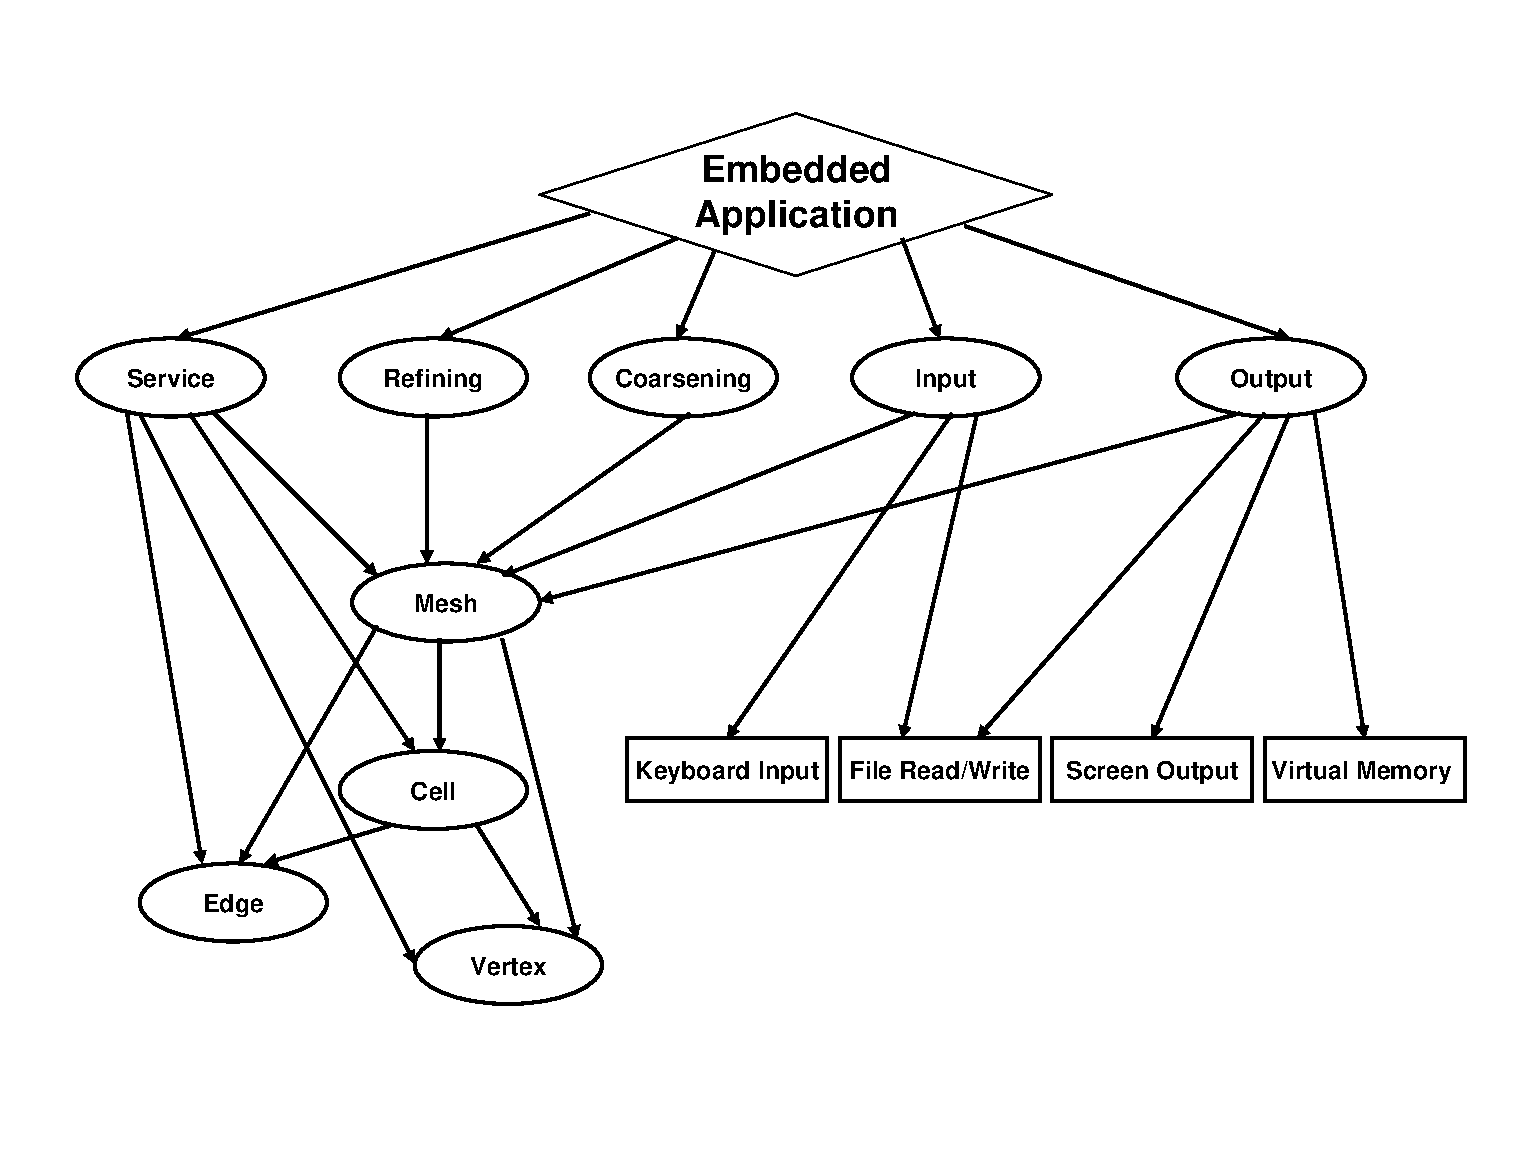
\includegraphics[width=0.90\textwidth]{uh.eps}
\caption{Use Hierarchy among Modules}
\label{fig:uh}
\end{figure}

\newpage

\bibliography{WenRef}
\bibliographystyle{plainnat}

\end{document}
